\documentclass{../kin_math}

\usepackage{wasysym}

\header{Elijah Kin}{Final Exam}{AMSC660}
\headrule

\begin{document}

\begin{questions}
  \question \textbf{Linear discriminant analysis} (LDA) (also known as \emph{Multiple Discriminant Analysis} (MDA)) is a linear dimensional reduction method aiming at projecting data from different categories to a low-dimensional space so that the images of data from different categories are separated as much as possible.

  Let $X$ be an $n \times d$ matrix whose rows are $d$-dimensional data points. We assume that the dataset consists of $c > 1$ categories. Let $\mathcal{I}_i$ denote the set of indices of data from category $i$, $i = 1, \dots , c$, and
  \begin{equation*}
    |\mathcal{I}_i| = n_i, \quad \mathcal{I}_i \cap \mathcal{I}_j = \varnothing, \quad \mathcal{I}_1 \cup \dots \cup \mathcal{I}_c = \{1, \dots, n\}.
  \end{equation*}
  We seek a $d \times d_1$ matrix $W$, $d_1 \leq c - 1$, that maps the data onto a $d_1$-dimensional space:
  \begin{equation}
    \label{eq:map}
    Y = XW, \quad \text{or}, \quad y_k = W^\top x_k, k = 1, \dots, n,
  \end{equation}
  such that images of the data from different categories under this mapping are separated as much as possible. In (\ref{eq:map}), $x_i \in \mathbb{R}^d$ is the $k$th row of $X$ written as a column vector. Likewise, is $y_k$.

  To pose this problem mathematically, we define the mean for each category in spaces $\mathbb{R}^d$ and $\mathbb{R}^{d_1}$,
  \begin{equation}
    m_i = \frac{1}{n_i} \sum_{k \in \mathcal{I}_i} x_k, \quad \tilde{m}_i = \frac{1}{n_i} \sum_{k \in \mathcal{I}_i} y_k = W^\top m_i, \quad i = 1, \dots, c.
  \end{equation}
  To describe the data variation within and between the categories, we define the \emph{within-class} and \emph{between-class scatter matrices} $S_w$ and $S_b$, respectively. These matrices are of size $d \times d$. The within-class scatter matrix is defined as
  \begin{equation}
    S_w \coloneqq \sum_{i = 1}^c S_i,
  \end{equation}
  where $S_i$ is the scatter matrix of category $i$ defined as
  \begin{equation}
    S_i \coloneqq \sum_{k \in \mathcal{I}_i} (x_k - m_i)(x_k - m_i)^\top \equiv (X_{\mathcal{I}_i,  :} - \textbf{1}_{n_i \times 1} m_i^\top)^\top (X_{\mathcal{I}_i, :} - \textbf{1}_{n_i \times 1} m_i^\top).
  \end{equation}
  The between-class scatter matrix is defined as
  \begin{equation}
    S_b \coloneqq \sum_{i = 1}^c n_i (m_i - m) (m_i - m)^\top, \quad \text{where} \quad m \coloneqq \frac{1}{n} \sum_{i = 1}^c n_i m_i \equiv \frac{1}{n} \sum_{k = 1}^n x_k
  \end{equation}
  is the overall mean. Note that the rank of $S_b$ is at most $c - 1$ as it is a sum of $c$ rank-1 matrices, and these matrices are not independent (see below).

  We use a similar notation with tilde on top for the mapped data. The within- and between-class scatter matrices for the mapped data are:
  \begin{equation}
    \tilde{S}_w = W^\top S_w W, \quad \tilde{S}_b = W^\top S_b W.
  \end{equation}
  Our goal is to find a $d \times d_1$ matrix $W$, mapping the data within each category into clusters and mapping the clusters corresponding to different categories as far as possible from each other. Therefore, we define the objective function as
  \begin{equation}
    J(w) = \frac{w^\top S_b w}{w^\top S_w w}.
  \end{equation}
  The function $J(w)$ is \textbf{maximized} by solving the \emph{generalized eigenvalue problem} (see below). It has at most $c - 1$ nonzero eigenvalues. We compose the matrix $W$ out of the eigenvectors corresponding to the top $d_1 \leq \textsf{rank}(S_b)$ eigenvalues.
  \begin{enumerate}[label=\arabic*.]
    \item Prove that the rank of $S_b$ is at most $c - 1$. \emph{Hint: Show that it can be represented as a sum of
    $c - 1$ rank-1 matrices.}
    \begin{solution}
      Observe first that
      \begin{equation*}
        \sum_{i = 1}^c n_i (m_i - m) = \sum_{i = 1}^c n_im_i - \sum_{i = 1}^c n_i m = nm - m \sum_{i = 1}^c n_i = nm - nm = 0,
      \end{equation*}
      so $\{m_i - m\}_{i = 1}^c$ is linearly dependent. Now, note that we can write
      \begin{multline}
        \label{eq:Sb}
        S_b = \sum_{i = 1}^c n_i (m_i - m) (m_i - m)^\top \\
        = \begin{bmatrix} \sqrt{n_1} (m_1 - m) & \dots & \sqrt{n_c} (m_i - m) \end{bmatrix} \begin{bmatrix} \sqrt{n_1} (m_1 - m)^\top \\ \vdots \\ \sqrt{n_c} (m_i - m)^\top \end{bmatrix}.
      \end{multline}
      For brevity, let $M$ be the $d \times c$ matrix
      \begin{equation*}
        M \coloneqq \begin{bmatrix} \sqrt{n_1} (m_1 - m) & \dots & \sqrt{n_c} (m_i - m) \end{bmatrix},
      \end{equation*}
      in which case we can rewrite (\ref{eq:Sb}) as $S_b = MM^\top$. From the fact that $\{m_i - m\}_{i = 1}^c$ is linearly dependent, we see that the columns of $M$ are linearly dependent, and hence $\textsf{rank}(M) \leq c - 1$.

      Finally, we claim that $\textsf{rank}(A^\top A) = \textsf{rank}(A)$ for any matrix $A$. To see this, we will show that $A^\top A x = 0$ if and only if $A x = 0$. First, if $Ax = 0$, then certainly $A^\top Ax = A^\top 0 = 0$. On the other hand, if $A^\top A x = 0$, then multiplying both sides by $x^\top$, we obtain
      \begin{equation*}
        x^\top A^\top A x = (Ax)^\top (Ax) = 0
      \end{equation*}
      and hence $Ax = 0$. Therefore, $\textsf{null}(A^\top A) = \textsf{null}(A)$, and so by the rank-nullity theorem, $\textsf{rank}(A^\top A) = \textsf{rank}(A)$ since $A^\top A$ and $A$ have the same number of columns. Hence, it follows that since $\textsf{rank}(A^\top) = \textsf{rank}(A)$,
      \begin{equation*}
        \textsf{rank}(S_b) = \textsf{rank}(MM^\top) = \textsf{rank}(M^\top) = \textsf{rank}(M) \leq c - 1
      \end{equation*}
      as desired.
    \end{solution}
    \item Assume that the within-class scatter matrix $S_w$ is nonsingular. Calculate the gradient of $J(w)$ with respect to $w$. Look at it attentively and show that the stationary points of $J(w)$ are those where
    \begin{equation}
      \label{eq:eigen}
      S_b w = \lambda S_w w.
    \end{equation}
    What are these values of $\lambda$? The problem of finding pairs $(\lambda, w)$ satisfying (\ref{eq:eigen}) is called the \emph{generalized eigenvalue problem}.
    \begin{solution}
      By the quotient rule, we have that
      \begin{multline*}
        \nabla J(w) = \frac{(w^\top S_w w) \nabla [w^\top S_b w] - (w^\top S_b w) \nabla [w^\top S_w w]}{(w^\top S_w w)^2} \\
        = \frac{2 (w^\top S_w w) S_b^\top w - 2 (w^\top S_b w) S_w^\top w}{(w^\top S_w w)^2}
      \end{multline*}
      and hence if $\nabla J(w) = 0$, then it must be that $(w^\top S_w w) S_b^\top w = (w^\top S_b w) S_w^\top w$. We divide both sides of this equation by $w^\top S_w w$ (which is nonzero provided $w \neq 0$ since $S_w$ is invertible) to yield
      \begin{equation*}
        S_b^\top w = \frac{w^\top S_b w}{w^\top S_w w} S_w^\top w = J(w) S_w^\top w.
      \end{equation*}
      Finally, note that $S_b$ and $S_w$ are both symmetric as they are sums of outer products, hence we obtain the generalized eigenvalue problem
      \begin{equation*}
        S_b w = J(w) S_w w
      \end{equation*}
      with $\lambda = J(w)$.
    \end{solution}
    \item Then use the Cholesky decomposition of $S_w$, $S_w = LL^\top$, to reduce the generalized eigenvalue problem to a symmetric eigenvalue problem of the form $A y = \lambda y$.
    \begin{solution}
      Substituting the Cholesky decomposition $S_w = LL^\top$ into the equation obtain, we obtain
      \begin{equation*}
        S_b w = J(w) LL^\top w.
      \end{equation*}
      Multiplying both sides by $L^{-1}$, we obtain
      \begin{equation*}
        L^{-1} S_b w = J(w) L^\top w.
      \end{equation*}
      Further, note that
      \begin{equation*}
        L^{-1} S_b = L^{-1} S_b I = L^{-1} S_b L^{-\top} L^\top
      \end{equation*}
      and hence
      \begin{equation*}
        L^{-1} S_b L^{-\top} L^\top w = J(w) L^\top w
      \end{equation*}
      and so by a change of variables $y = L^\top w$, we obtain the symmetric eigenvalue problem
      \begin{equation*}
        L^{-1} S_b L^{-\top} y = J(w) y,
      \end{equation*}
      so $y$ are eigenvectors of $L^{-1} S_b L^{-\top}$. Once we find these eigenvectors, we can easily recover the desired $w = L^{-\top} y$.
    \end{solution}
    \item Apply LDA to the MNIST set of training images of 3, 8, and 9. Thus, you have a dataset consisting of three categories. Hence, $S_b$ has most rank 2. Solve the arising generalized eigenvalue problem using the standard functions in Matlab or Python. Display the mapped training data of 3, 8, and 9 in 2D colored in three different colors, respectively. Include legend.
    You should see that the result is quite good\smiley.
    \begin{solution}
      We implement the LDA mapping for the MNIST dataset in the code \href{https://github.com/elijahkin/amsc660/blob/main/final/final.ipynb}{here}, and provide the mapping below. The result indeed seems quite good.
      \begin{figure}
        \centering
        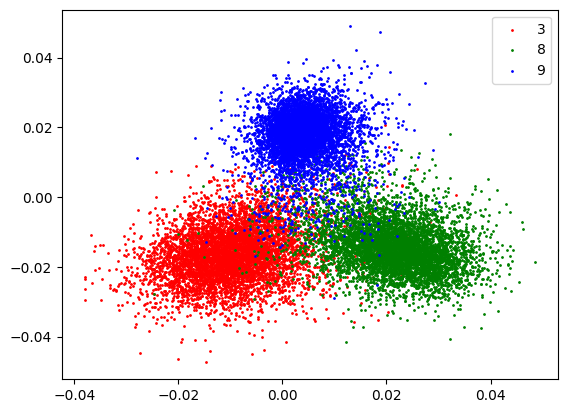
\includegraphics[scale=0.65]{mnist_lda.png}
        \caption{LDA Mapping}
      \end{figure}
    \end{solution}
    \item For comparison, map the MNIST set of training images of 3, 8, and 9 onto the first two PCAs (the top two right singular vectors of the centered data matrix $X - \textbf{1}_{n \times 1} m^\top$). You will see that this mapping mixes the images of 3, 8, and 9 much more.
    \begin{solution}
      We plot the mapping onto the first two PCAs below. Indeed, we find that this mapping has more mixing than the LDA mapping above, as expected.
      \begin{figure}
        \centering
        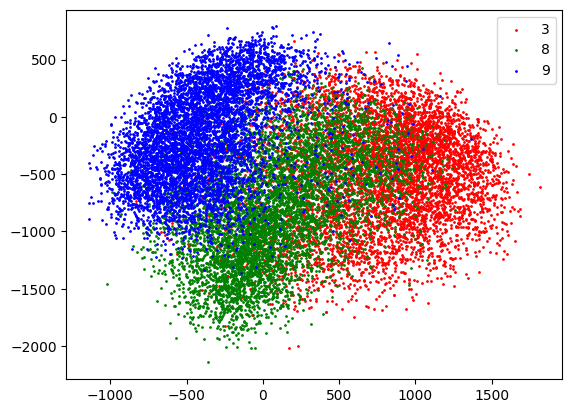
\includegraphics[scale=0.65]{mnist_pca.png}
        \caption{PCA Mapping}
      \end{figure}
    \end{solution}
  \end{enumerate}

  \question \emph{In this problem, you should show your knowledge of optimization algorithms and the ability to apply them. I provide the function and its gradient, a plotting function, and a few auxiliary functions.}
  \begin{figure}
    \centering
    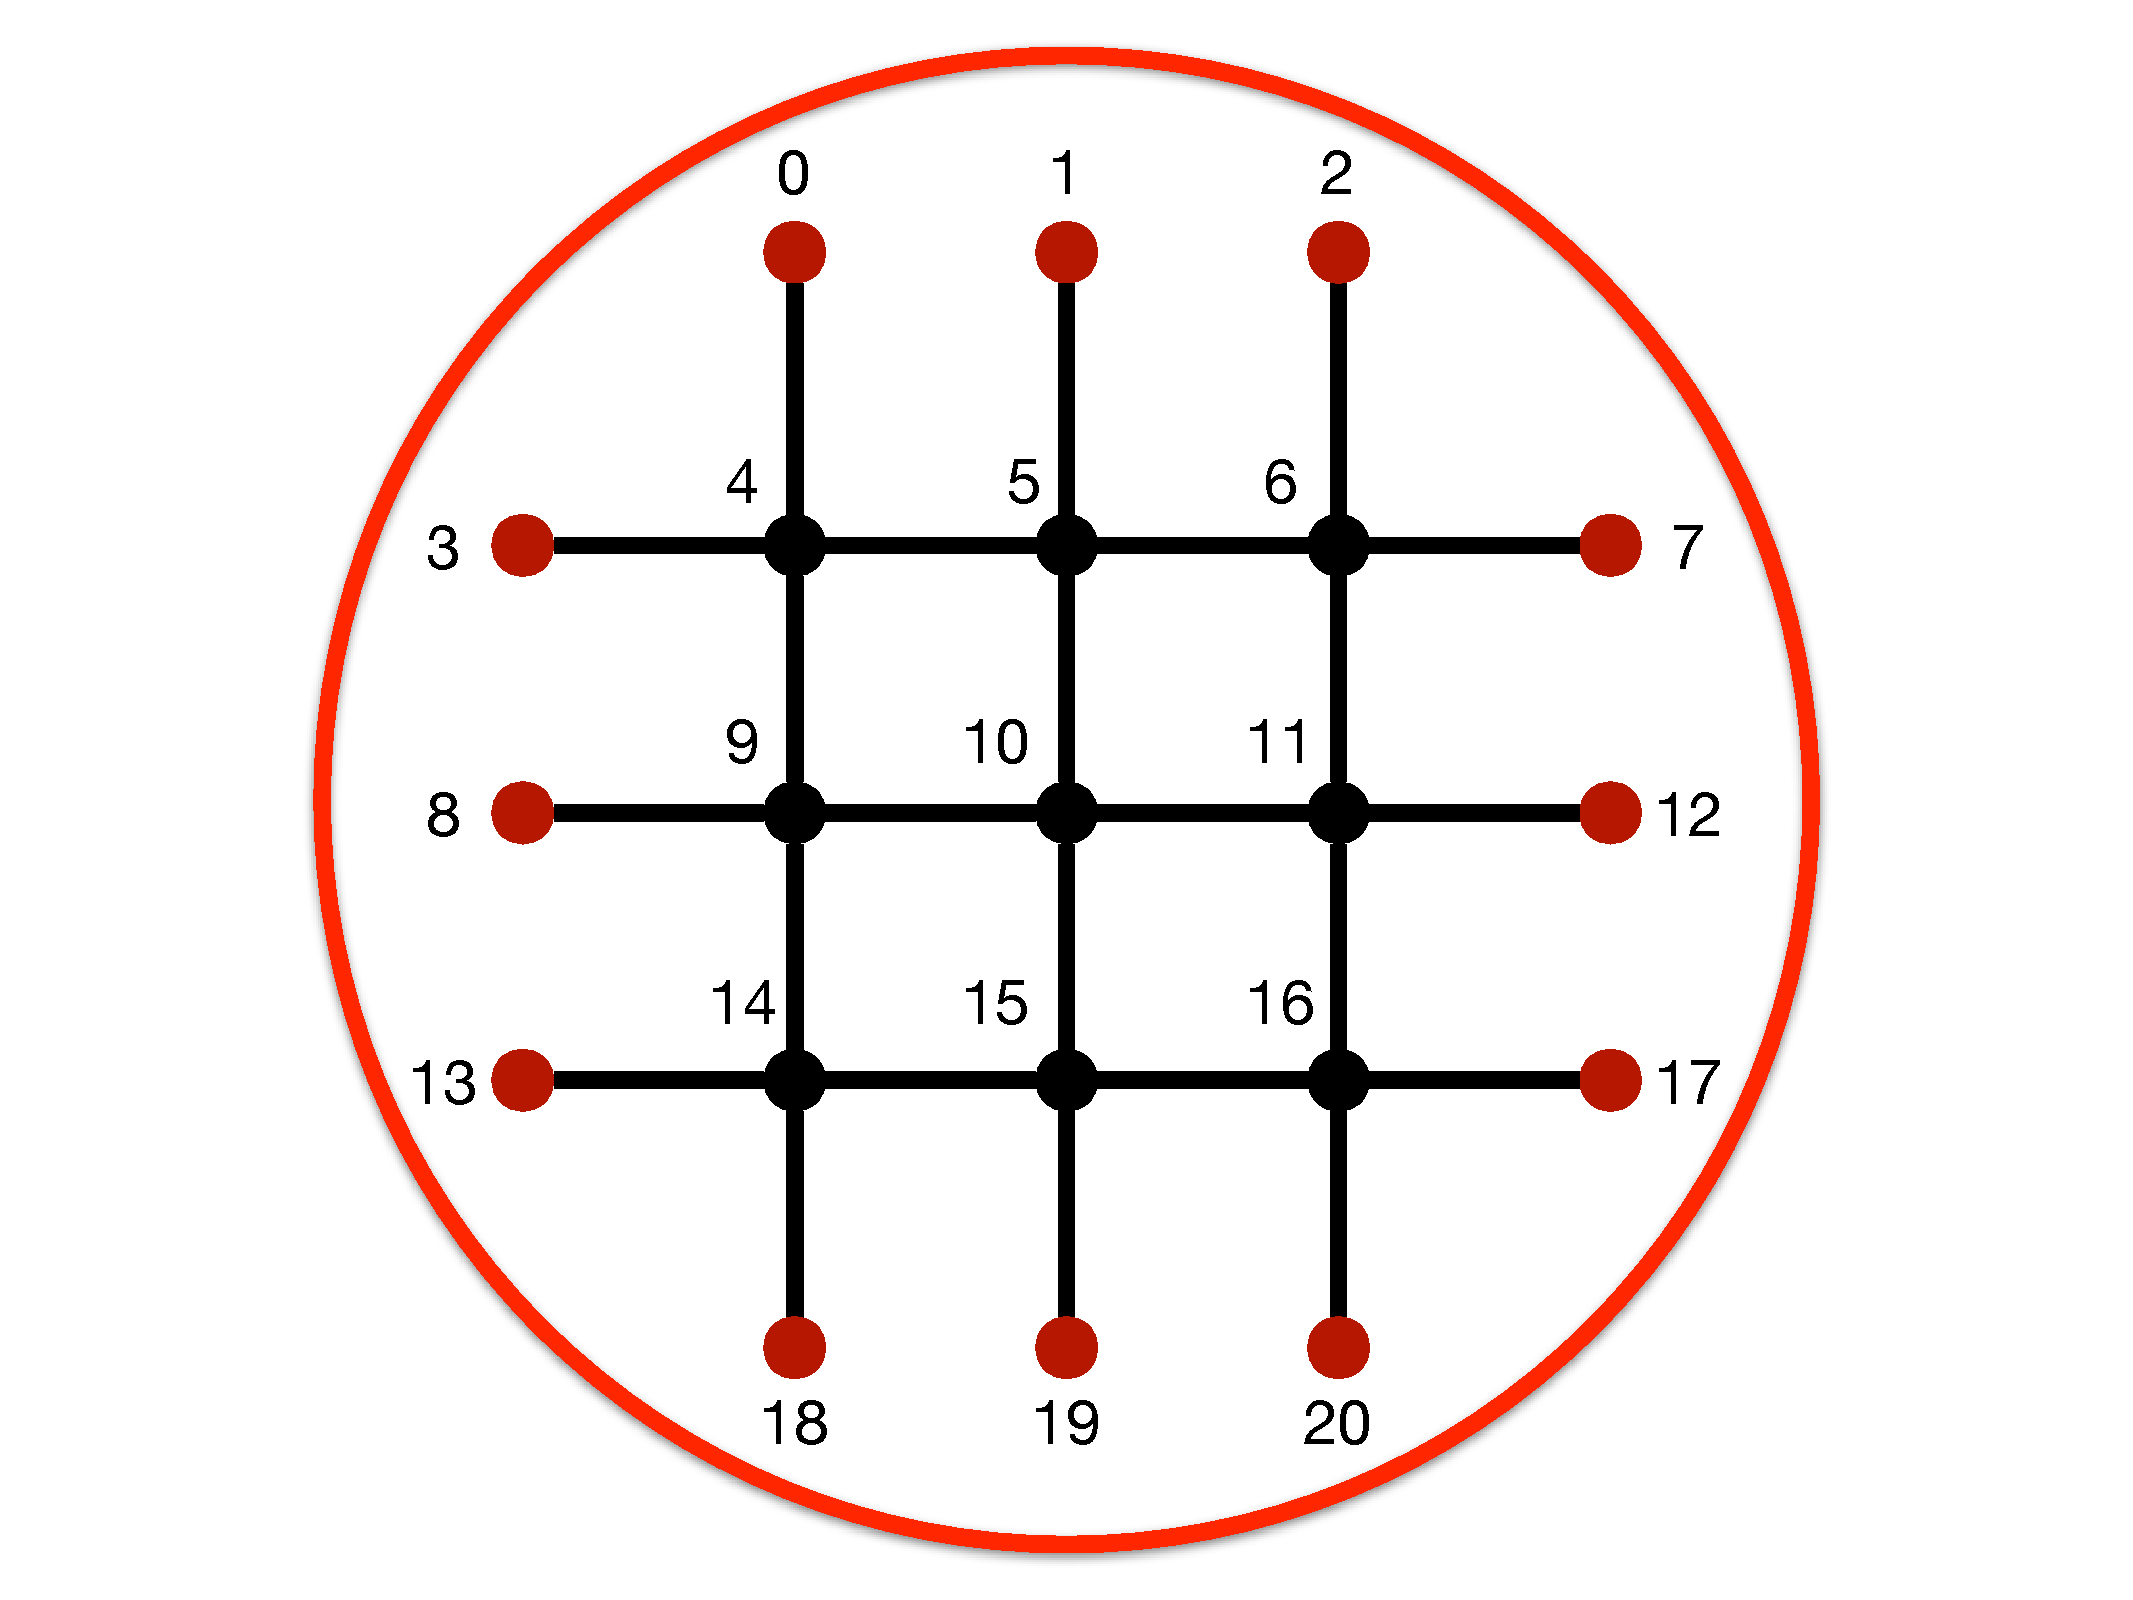
\includegraphics[scale=0.2]{springs.pdf}
    \label{fig:springs}
    \caption{The spring system in Problem 2.}
  \end{figure}
  Suppose you have a spring system consisting of 21 nodes and 24 springs, see Fig. 1. Imagine that you need to attach the red nodes to a hoop so that the total spring energy at equilibrium is minimal. The radius of the hoop is $R = 3$. The equilibrium length of each spring is $r_0 = 1$, and the spring constant of each spring is $\kappa = 1$. The energy of the spring system is
  \begin{equation}
    E = \frac{\kappa}{2} \sum_\textsf{spring} \left(\| \textbf{r}_{\textsf{spring}[0]} - \textbf{r}_{\textsf{spring}[1]} \| - r_0\right)^2
  \end{equation}
  where the sum is taken over all springs, and $\textbf{r}_{\textsf{spring}[0]}$ and $\textbf{r}_{\textsf{spring}[1]}$ denote the $(x, y)$-coordinates of the endpoints of the spring.

  Since the positions of the 12 red nodes must be on the hoop, they are defined by their angles on the hoop. The 9 black nodes are free. Their positions are described by their $(x, y)$ coordinates.Thus, we need to optimize the energy with respect to 12 + 9 + 9 = 30 parameters, the first 12 of which are the angles of the red nodes, the next 9 are the $x$-coordinates of the black nodes, and the last 9 are the $y$-coordinates of the black nodes.

  The derivative of the energy with respect to the angle $\theta_i$ of a red node $i$ is
  \begin{equation}
    \frac{\partial E}{\partial \theta_i} = \kappa R(\|\textbf{r}_i - \textbf{r}_j\| - r_0) \frac{-x_i \sin \theta_i + y_i \cos \theta_i}{\|\textbf{r}_i - \textbf{r}_j\|},
  \end{equation}
  where $j$ is the unique node connected to the red node $i$ by a spring. The derivatives of the energy with respect to $x_i$ and $y_i$, the $x$- and $y$-coordinates of a black node $i$, are, respectively
  \begin{equation}
    \frac{\partial E}{\partial x_i} = \kappa \sum_{j \sim i} (\|\textbf{r}_i - \textbf{r}_j\| - r_0) \frac{x_i}{\|\textbf{r}_i - \textbf{r}_j\|},
  \end{equation}
  \begin{equation}
    \frac{\partial E}{\partial y_i} = \kappa \sum_{j \sim i} (\|\textbf{r}_i - \textbf{r}_j\| - r_0) \frac{y_i}{\|\textbf{r}_i - \textbf{r}_j\|},
  \end{equation}
  where the summation is over all nodes $j$ connected to the black node $i$ by springs.

  \textbf{Task:}
  \begin{itemize}
    \item Implement any \textbf{two different} optimization methods to find the minimal value of the spring energy.
    \begin{solution}
      Taking inspiration from homework 13, we implement Nesterov's accelerated descent (NAG) and Adam; the code for these can be found \href{https://github.com/elijahkin/amsc660/blob/main/final/final.ipynb}{here}.
    \end{solution}
    \item Plot the spring energy and the norm of its gradient versus the iteration number for each method.
    \begin{solution}
      We plot below the results of running NAG for 100 iterations with a step size of $\alpha = 0.1$, and also running Adam for 250 iterations with a step size of $\alpha = 2 \cdot 10^{-2}$ and the other hyperparameters as suggested ($\beta_1 = 0.9$, $\beta_2 = 0.999$, and $\epsilon = 10^{-8}$).
      \begin{figure}
        \centering
        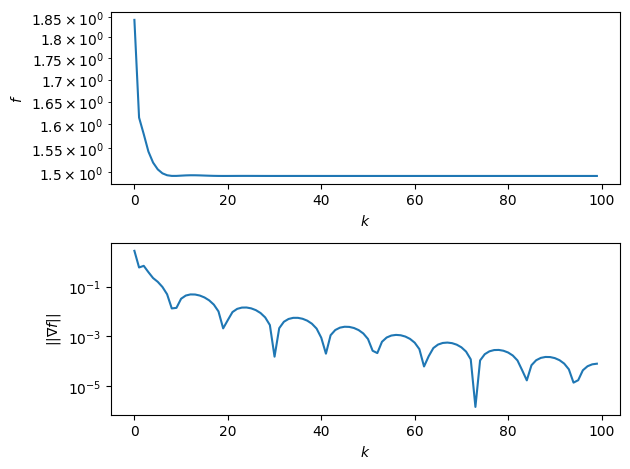
\includegraphics[scale=0.47]{nest_plots.png}
        \caption{Plots for NAG}
      \end{figure}
      \begin{figure}
        \centering
        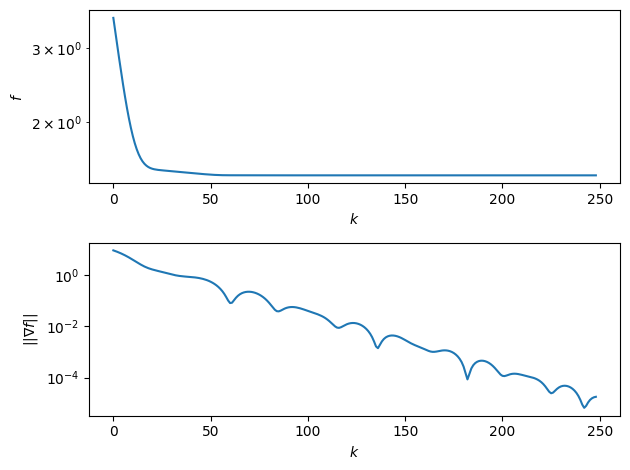
\includegraphics[scale=0.47]{adam_plots.png}
        \caption{Plots for Adam}
      \end{figure}
      As we would like, in both cases the plot of the energy flattens out, while the norm of the gradient approaches 0. Note that the scale of the $y$-axis in all plots is logarithmic.
    \end{solution}
    \item Plot the resulting view of the spring system stretched on the hoop for each method.
    \begin{solution}
      We plot below the view of spring system for the minima found by each method. As we would wish, the two agree.
      \begin{figure}
        \centering
        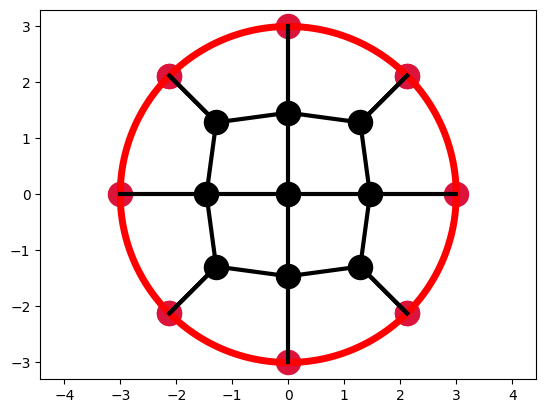
\includegraphics[scale=0.6]{nest_springs.png}
        \caption{Spring System for NAG}
      \end{figure}
      \begin{figure}
        \centering
        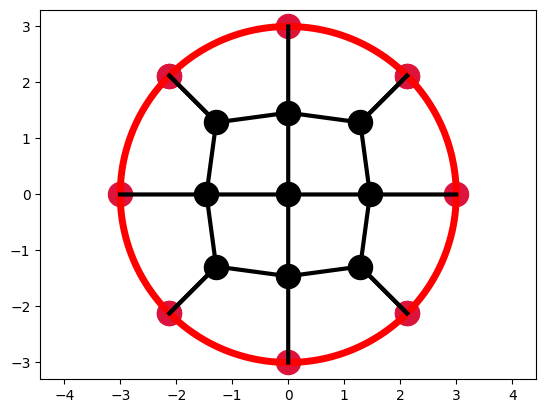
\includegraphics[scale=0.6]{adam_springs.png}
        \caption{Spring System for Adam}
      \end{figure}
    \end{solution}
    \item Print the positions of the nodes, the resulting energy, and the norm of the gradient for each method.
    \begin{solution}
      With NAG, we achieve a final energy of $1.49245$ and a final norm of the gradient of $7.80845 \cdot 10^{-5}$. Similarly, with Adam, we achieve a final energy of $1.49245$ and a final norm of the gradient of $1.78081 \cdot 10^{-5}$. The positions of the nodes for each method are also printed \href{https://github.com/elijahkin/amsc660/blob/main/final/final.ipynb}{here}.
    \end{solution}
  \end{itemize}
  \textbf{Some useful arrays and functions.}
  \begin{itemize}
    \item The enumeration of the nodes in Python is shown in Fig. 1. The enumeration in Matlab is shifted by 1. Below I refer to the indexing and functions in Python. The functions in Matlab are similar though slightly adjusted for Matlab specifics.
    \item \texttt{Asymm} is the adjacency matrix of the spring system. \texttt{A} is its superdiagonal part.
    \item \texttt{ind\_hoop} is the list of indices of the hoop nodes (the red nodes).
    \item \texttt{ind\_free} is the list of indices of the free nodes (the black nodes).
    \item \texttt{springs} is a $2 \times 24$ array whose columns are the indices of the spring end nodes.
    \item Function \texttt{draw\_spring\_system(pos, springs, R, ind\_hoop, ind\_free)} plots the spring system stretched on the hoop.
    \item Function \texttt{compute\_gradient(theta, pos, Asymm, r0, kappa, R, ind\_hoop, ind\_free)} computes the gradient of the energy function.
    \item Function \texttt{Energy(theta, pos, springs, r0, kappa)} computes the energy function.
    \item Function \texttt{vec\_to\_pos(vec)} converts the vector of parameters,
    \begin{align*}
      \texttt{vec} = [ &\theta_0, \theta_3, \theta_8, \theta_{13}, \theta_{18}, \theta_{19}, \theta_{20}, \theta_{17}, \theta_{12}, \theta_7, \theta_2, \theta_1, \\
                       &x_4, x_5, x_6, x_9, x_{10}, x_{11}, x_{14}, x_{15}, x_{16}, y_4, y_5, y_6, y_9, y_{10}, y_{11}, y_{14}, y_{15}, y_{16} ],
    \end{align*}
    to the vector of angles \texttt{theta} of the red nodes and $21 \times 2$ array \texttt{pos} of $(x, y)$ coordinates of all nodes.
    \item Function \texttt{gradient(vec)} evaluates the energy gradient given the vector of parameters as input. It is created for use in the optimization routine. It calls \texttt{vec\_to\_pos(vec)} and \texttt{compute\_gradient(theta, pos, Asymm, r0, kappa, R, ind\_hoop, ind\_free)}.
    \item Function \texttt{func(vec)} evaluates the energy function given the vector of parameters as input. It is created for use in the optimization routine. It calls \texttt{vec\_to\_pos(vec)} and \texttt{Energy(theta, pos, springs, r0, kappa)}.
  \end{itemize}

  \question The unit cube in $\mathbb{R}^d$ centered at the origin is the set
  \begin{equation}
    C^d = \left\{ \textbf{x} \in \mathbb{R}^d \mid \max_{1 \leq i \leq d} |x_i| \leq \frac{1}{2} \right\},
  \end{equation}
  while the unit ball in $\mathbb{R}^d$ centered at the origin is the set
  \begin{equation}
    B^d = \left\{ \textbf{x} \in \mathbb{R}^d \mid \sum_{i = 1}^d x_i^2 \leq 1 \right\}.
  \end{equation}
  Obviously, all centers of the $(d - 1)$-dimensional faces of $C^d$, i.e., the points with one
  coordinate $\pm \frac{1}{2}$ and the rest zeros, lie inside $B^d$. The most remote points of $C^d$ from the origin are the corners with all coordinates $\pm \frac{1}{2}$. The distance of the corner of $C^d$ from the origin is $\sqrt{d} / 2$. For $d \geq 5$, the corners of $C^d$ and some of their neighborhoods lie outside $B^d$. The $d$-dimensional volume of $C^d$ is one, while the volume of $B^d$ is
  \begin{equation}
    \operatorname{Vol}\left(B^d\right) = \dfrac{\pi^{d / 2}}{\frac{d}{2} \Gamma\left(\frac{d}{2}\right)}.
  \end{equation}
  $\operatorname{Vol}\left(B^d\right)$ tends to zero as $d \to \infty$. Hence, the fraction of the unit cube $C^d$ lying inside $B^d$ also tends to zero as $d \to \infty$. You can read about this in more detail and see some illustrations e.g. \href{https://www.cs.cmu.edu/~venkatg/teaching/CStheory-infoage/chap1-high-dim-space.pdf}{here} (read at least up to Section 1.2.2 inclusively).

  Calculate
  \begin{equation}
    \operatorname{Vol}\left(B^d \cap C^d\right) \text{ in } d = 5, 10, 15, 20
  \end{equation}
  using Monte Carlo integration in two ways.
  \begin{enumerate}[label=\arabic*.]
    \item Way one uses a sequence of independent uniformly distributed random variables in the unit cube $C^d$.
    \begin{solution}
      Let $\Omega = B^d \cap C^d$. We first note that
      \begin{equation*}
        \operatorname{Vol}(\Omega) = \int_\Omega dx = \int_{C^d} g(x) \, dx
      \end{equation*}
      where $g(x)$ denotes the indicator function of $B^d$,
      \begin{equation*}
        g(x) = \begin{cases} 1 & x \in B^d \\ 0 & x \notin B^d \end{cases}.
      \end{equation*}
      Now suppose that $\eta$ is uniformly distributed in $C^d$ with pdf $f_\eta(x)$, so that
      \begin{equation*}
        \operatorname{Vol}(\Omega) = \int_{C^d} g(x) \, dx = \int_{C^d} \frac{g(x)}{f_\eta(x)} f_\eta(x) \, dx = \mathbb{E}_\eta \left[\frac{g(x)}{f_\eta(x)}\right],
      \end{equation*}
      and so further by the strong law of large numbers,
      \begin{equation*}
        \operatorname{Vol}(\Omega) = \mathbb{E}_\eta \left[\frac{g(x)}{f_\eta(x)}\right] \approx \frac{1}{N} \sum_{i = 1}^N \frac{g(\eta_i)}{f_\eta(\eta_i)}
      \end{equation*}
      where $\eta_i$, $1 \leq i \leq N$ are samples of $\eta$. Then since $\eta$ is uniformly distributed in $C^d$,
      \begin{equation*}
        \operatorname{Vol}(\Omega) \approx \frac{1}{N} \sum_{i = 1}^N \frac{g(\eta_i)}{f_\eta(\eta_i)} = \operatorname{Vol}(C^d) \frac{1}{N} \sum_{i = 1}^N g(\eta_i),
      \end{equation*}
      and since we are given that $\operatorname{Vol}(C^d) = 1$,
      \begin{equation*}
        \operatorname{Vol}(\Omega) \approx \frac{1}{N} \sum_{i = 1}^N g(\eta_i) = \frac{1}{N} \sum_{i = 1}^N \begin{cases} 1 & \eta_i \in B^d \\ 0 & \eta_i \notin B^d \end{cases}.
      \end{equation*}
      We use this approximation to estimate $\operatorname{Vol}(\Omega)$ \href{https://github.com/elijahkin/amsc660/blob/main/final/final.ipynb}{here}, finding the following values:
      \begin{itemize}
        \item $0.9996$ for $d = 5$
        \item $0.7627$ for $d = 10$
        \item $0.1973$ for $d = 15$
        \item $0.0182$ for $d = 20$
      \end{itemize}
    \end{solution}
    \item Way two uses a sequence of independent uniformly distributed random variables in the unit ball $B^d$. (You need to think of a way to generate such a random variable.)
    \begin{solution}
      As before, let $\Omega = B^d \cap C^d$, but now let $g(x)$ be the indicator function
      \begin{equation*}
        g(x) = \begin{cases} 1 & x \in C^d \\ 0 & x \notin C^d \end{cases}
      \end{equation*}
      for $C^d$. Then by an analogous argument to the above,
      \begin{equation*}
        \operatorname{Vol}(\Omega) = \int_\Omega dx = \int_{B^d} g(x) \, dx,
      \end{equation*}
      and so if $\eta$ is uniformly distributed in $B^d$ with pdf $f_\eta(x)$, then
      \begin{equation*}
        \operatorname{Vol}(\Omega) = \int_{B^d} g(x) \, dx = \int_{B^d} \frac{g(x)}{f_\eta(x)} f_\eta(x) \, dx = \mathbb{E}_\eta \left[\frac{g(x)}{f_\eta(x)}\right].
      \end{equation*}
      Hence, by the strong law of large numbers,
      \begin{equation*}
        \operatorname{Vol}(\Omega) = \mathbb{E}_\eta \left[\frac{g(x)}{f_\eta(x)}\right] \approx \frac{1}{N} \sum_{i = 1}^N \frac{g(\eta_i)}{f_\eta(\eta_i)} = \operatorname{Vol}(B^d) \frac{1}{N} \sum_{i = 1}^N g(\eta_i)
      \end{equation*}
      where $\eta_i$, $1 \leq i \leq N$ are samples of $\eta$. Recall we are given that
      \begin{equation*}
        \operatorname{Vol}(B^d) = \frac{\pi^{d / 2}}{\frac{d}{2} \Gamma\left(\frac{d}{2}\right)}
      \end{equation*}
      and so
      \begin{equation*}
        \operatorname{Vol}(\Omega) \approx \frac{\pi^{d / 2}}{\frac{d}{2} \Gamma\left(\frac{d}{2}\right)} \frac{1}{N} \sum_{i = 1}^N \begin{cases} 1 & \eta_i \in C^d \\ 0 & \eta_i \notin C^d \end{cases}.
      \end{equation*}
      We use this approximation to estimate $\operatorname{Vol}(\Omega)$ via the code \href{https://github.com/elijahkin/amsc660/blob/main/final/final.ipynb}{here}. To sample uniformly in $B^d$, we first generate a uniformly distributed point on its boundary, via
      \begin{equation*}
        \frac{\xi}{\sqrt{\xi_1^2 + \dots + \xi_d^2}}
      \end{equation*}
      where $\xi \sim \mathcal{N}(0, 1)$ as discussed in class. This establishes a direction, but it remains to establish a radius. We generate $\eta \sim \mathcal{U}[0, 1]$ and pick $\eta^{1 / d}$ to account for the larger surface area of larger radii. We find the following values, which generally agree with the corresponding values found above:
      \begin{itemize}
        \item $0.9996$ for $d = 5$
        \item $0.7625$ for $d = 10$
        \item $0.1972$ for $d = 15$
        \item $0.0182$ for $d = 20$
      \end{itemize}
    \end{solution}
  \end{enumerate}

\end{questions}

\end{document}
